\section{Introduction}
As robots are tasked with challenges of ever-increasing complexity, the need
for a hierarchical system of planning for a goal becomes evident. Such systems
draw clear parallels to the way we plan our own actions: rather than
immediately thinking about the individual muscle motions required to achieve a particular
goal, we apply a top-down approach, first considering at a high level the
steps to be taken, then refining these to lower levels. Recent methods for
hierarchical planning consider the intersection of high-level task planning
and low-level motion planning. In this framework, the (classical) task planner produces
a symbolic plan containing the necessary sequence of actions to reach a goal
state, and an interface layer refines this plan by sampling values for
the symbols, thus grounding the plan. The two central challenges in building such
an interface layer are designing good distributions from which to sample
pose values for the symbolic plan parameters and refining the parameters using a
well-performing algorithm.

\begin{figure}[h]
  \centering
    \noindent
    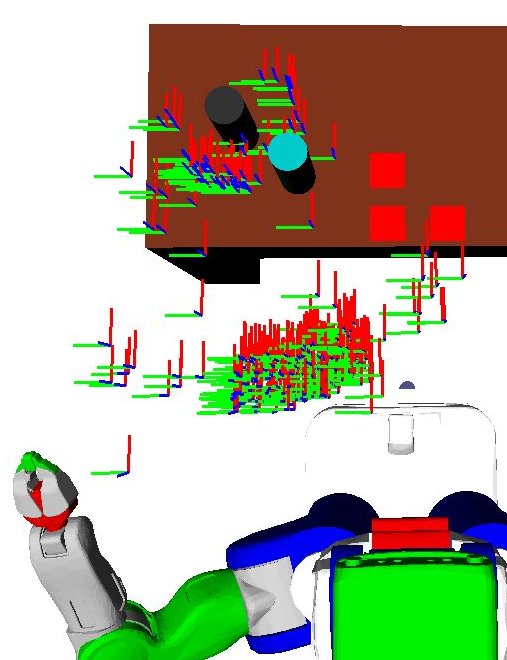
\includegraphics[scale=0.2]{images/move_grasp.png}\hspace{10 mm}
    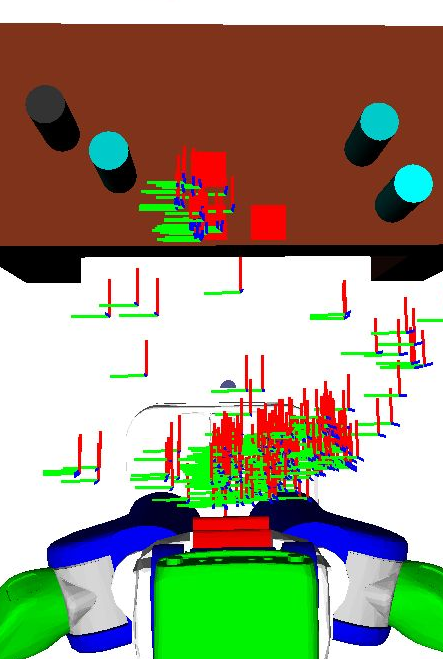
\includegraphics[scale=0.2]{images/move_putdown.png}
  \caption{Screenshots showing some distributions learned by our system in one experimental
    setup. The robot is tasked with grasping the black cylinder and putting it down on the
    central red square. The left image shows learned base motion and grasping distributions,
    and the right shows learned base motion and putdown distributions. The grasp distribution
    properly learned to avoid the region close to the blue obstruction. We sample from these distributions
    to refine the high-level plan, rather than relying on hand-coded generators.}
  \label{fig:cover}
\end{figure}

Our work improves directly upon the interface layer built
by Srivastava et al. They propose a complete backtracking search algorithm for refining
the high-level plan into a set of collision-free trajectories using motion planning, or
propagating symbolic error information back to the task planner if this is not possible.

This restriction has several negative implications: these
constants must be fine-tuned when running the system in a new setting, and the
resulting refinement distributions are primitive.

implications of hand coded generators